\section{LLA}
LLA coordinates (longitude, lattitude, attitude) are the more intuitive way to express a position on the earth's surface. The values ``longitude'' and ``lattitude'' are angles and therefore in degrees or radians and the ``attitude'' is in meters above the surface of the earth's approximated shape. 

\begin{figure}[h!]
	\centering
	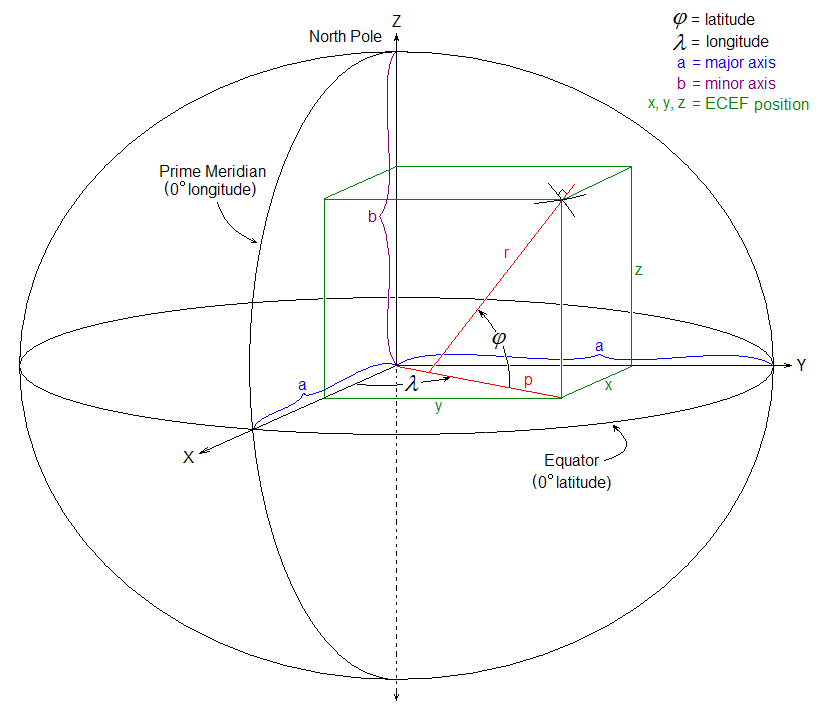
\includegraphics[width=10cm]{ECEF}
	\caption{LLA coordinates}
	\label{LLA coordinates1}
\end{figure}

LLA coordinates are defined using
\begin{equation}
p_{LLA} = \begin{pmatrix} \lat \\ \lon \\ h \end{pmatrix}
\end{equation}
available for the following simple types
\begin{itemize}
\item int32\_t - \texttt{LlaCoor\_i}
\item float - \texttt{LlaCoor\_f}
\item double - \texttt{LlaCoor\_d}
\end{itemize}

\subsection{Simple Operations}
\subsubsection*{Assigning}
It is either possible to assign every single value of LLA-coordinate
\begin{equation}
pos = \begin{pmatrix}	\lat	\\
						\lon	\\
						h		\end{pmatrix}
\end{equation}
\inHfile{LLA\_ASSIGN(pos, lat, lon, alt)}{pprz\_geodetic}

\noindent
or to copy one coordinate to another

\texttt{pos1 = pos2}\\
\inHfile{LLA\_COPY(pos1, pos2)}{pprz\_geodetic}


\subsection{Trasnformation from LLA}
\subsubsection*{to ECEF}
Calculating the ECEF coordinates out of LLA coordinates is a slightly easier task than the other way round. The following way refers to \cite{wiki:1}. With the known constants
\begin{align}
a	&= 6,378,137				\\
f	&= \frac{1}{298.257223563}	\\
e^2	&= \sqrt{2f-f^2}			
\end{align}
the value
\begin{equation}
\chi = \sqrt{1-e^2\sin^2 \lat}
\end{equation}
can be precomputed and used in
\begin{align}
x &= \left(\tfrac a \chi + h \right) \cos \lat \cos \lon \\
y &= \left(\tfrac a \chi + h \right) \cos \lat \sin \lon \\
z &= \left(\tfrac a \chi (1-e^2) + h \right) \sin \lat
\end{align}
\inCfile{ecef\_of\_lla\_i(EcefCoor\_i* out, LlaCoor\_i* in)}{pprz\_geodetic\_int}
\inCfile{ecef\_of\_lla\_f(EcefCoor\_f* out, LlaCoor\_f* in)}{pprz\_geodetic\_float}
\inCfile{ecef\_of\_lla\_d(EcefCoor\_d* ecef, LlaCoor\_d* lla)}{pprz\_geodetic\_double}


\subsection{Transforming to LLA}
\subsubsection*{from ECEF}
Generating LLA coordinates is made using the following calculations. These refer to \cite{wiki:1} or \cite{Wendel__2007}(pages 31-33).

\begin{align}
a	&= 6,378,137										\\
f	&= \frac{1}{298.257223563}							
\end{align}
\begin{align}
b	&= a \multiplication (1-f)							\\
e^2	&= \sqrt{2f-f^2}									\\
e'	&= e \frac{a}{b}									\\
E^2	&= a^2-b^2											\\
r	&= \sqrt{ x^2 + y^2}								\\
F	&= 54 b^2 z^2										\\
G	&= r^2 + (1-e^2)z^2-e^2E^2							\\
c	&= \frac{e^4Fr^2}{G^3}								\\
s	&= \sqrt[3]{1+c+\sqrt{c^2+2c}}						\\
P	&= \frac{F}{3\left(s+\tfrac 1 s + 1\right)^2 G^2}	\\
Q	&= \sqrt{1+2e^4P}									\\
r_0	&= -\frac{Pe^2r}{1+Q} + \sqrt{\tfrac 1 2 a^2 \left(1 + \tfrac 1 Q \right) - \frac{P(1-e^2)z^2}{Q(1+Q)}-\tfrac 1 2 P r^2}	\\
U	&= \sqrt{(r-e^2r_0)^2+z^2}							\\
V	&= \sqrt{(r-e^2r_0)^2+(1-e^2)z^2}					\\
z_0	&= \frac{b^2z}{aV}									\\
\lat	&= \arctan \left( \frac{z+(e')^2z_0} r \right)	\\
\lon	&= atan2(y,x)									\\
h	&= U \left( \frac{b^2}{aV} - 1 \right)
\end{align}
\inCfile{lla\_of\_ecef\_i(LlaCoor\_i* out, EcefCoor\_i* in)}{pprz\_geodetic\_int}
\inCfile{lla\_of\_ecef\_f(LlaCoor\_f* out, EcefCoor\_f* in)}{pprz\_geodetic\_float}
\inCfile{lla\_of\_ecef\_d(LlaCoor\_d* lla, EcefCoor\_d* ecef)}{pprz\_geodetic\_double}